\section{Введение}

В данной лабораторной работе рассматриваются методы линеаризации обратной связью для нелинейных систем управления. Основное внимание уделяется анализу линеаризуемости по входу-выходу, преобразованию систем в нормальную форму и синтезу законов управления.

Основные задачи работы:
\begin{enumerate}
\item Анализ линеаризуемости по входу-выходу нелинейной системы
\item Преобразование системы в нормальную форму с указанием области определения
\item Проверка минимально-фазовости системы
\item Синтез закона управления методом линеаризации обратной связью для глобальной стабилизации
\end{enumerate}

Работа демонстрирует применение теоретических методов линеаризации обратной связью к практическим задачам управления нелинейными системами.

\section{Задача 1. Анализ линеаризуемости по входу-выходу}

Рассмотрим систему:
\begin{align}
\dot{x}_1 &= -x_1 + x_2 - x_3 \\
\dot{x}_2 &= -x_1 x_3 - x_2 + u \\
\dot{x}_3 &= -x_1 + u \\
y &= x_3
\end{align}

\subsection{Проверка линеаризуемости по входу-выходу}

Для проверки линеаризуемости по входу-выходу вычислим производные Ли выходной функции $h(x) = x_3$.

\textbf{Шаг 1:} Вычисление производных Ли
\begin{align}
L_f^0 h &= h = x_3 \\
L_f^1 h &= \frac{\partial h}{\partial x_1} f_1 + \frac{\partial h}{\partial x_2} f_2 + \frac{\partial h}{\partial x_3} f_3 \\
&= 0 \cdot (-x_1 + x_2 - x_3) + 0 \cdot (-x_1 x_3 - x_2) + 1 \cdot (-x_1 + u) \\
&= -x_1 + u
\end{align}

\textbf{Шаг 2:} Проверка условия линеаризуемости
\begin{align}
L_g L_f^0 h &= \frac{\partial h}{\partial x_1} g_1 + \frac{\partial h}{\partial x_2} g_2 + \frac{\partial h}{\partial x_3} g_3 \\
&= 0 \cdot 0 + 0 \cdot 1 + 1 \cdot 1 = 1 \neq 0
\end{align}

Поскольку $L_g L_f^0 h = 1 \neq 0$, система линеаризуема по входу-выходу с относительной степенью $r = 1$.

\subsection{Преобразование в нормальную форму}

Для системы размерности $n = 3$ с относительной степенью $r = 1$ размерность внутренней динамики равна $n - r = 2$.

\textbf{Координаты нормальной формы:}
\begin{align}
z_1 &= h = x_3 \\
z_2 &= L_f h = -x_1 + u
\end{align}

\textbf{Внутренние координаты:}
\begin{align}
\eta_1 &= x_1 \\
\eta_2 &= x_2
\end{align}

\textbf{Производные координат нормальной формы:}
\begin{align}
\dot{z}_1 &= \dot{x}_3 = -x_1 + u \\
\dot{z}_2 &= \frac{d}{dt}(L_f h) = \frac{d}{dt}(-x_1 + u) = -\dot{x}_1 + \dot{u} \\
&= -(-x_1 + x_2 - x_3) + \dot{u} = x_1 - x_2 + x_3 + \dot{u}
\end{align}

\textbf{Область определения преобразования:}
Преобразование определено для всех $x \in \mathbb{R}^3$. Обратное преобразование:
\begin{align}
x_1 &= \eta_1 \\
x_2 &= \eta_2 \\
x_3 &= z_1
\end{align}

\subsection{Проверка минимально-фазовости}

Для проверки минимально-фазовости анализируем внутреннюю динамику при нулевом выходе $y = z_1 = 0$.

При $y = 0$ имеем $x_3 = 0$. Внутренняя динамика при $x_3 = 0$:
\begin{align}
\dot{x}_1 &= -x_1 + x_2 \\
\dot{x}_2 &= -x_1 \cdot 0 - x_2 + u = -x_2 + u
\end{align}

При $u = 0$:
\begin{align}
\dot{x}_1 &= -x_1 + x_2 \\
\dot{x}_2 &= -x_2
\end{align}

Матрица линеаризации внутренней динамики:
\begin{equation}
A = \begin{pmatrix} -1 & 1 \\ 0 & -1 \end{pmatrix}
\end{equation}

Собственные значения: $\lambda_1 = -1$, $\lambda_2 = -1$.

Поскольку все собственные значения имеют отрицательную вещественную часть, система минимально-фазовая.

\subsection{Моделирование системы}

\begin{figure}[H]
\centering
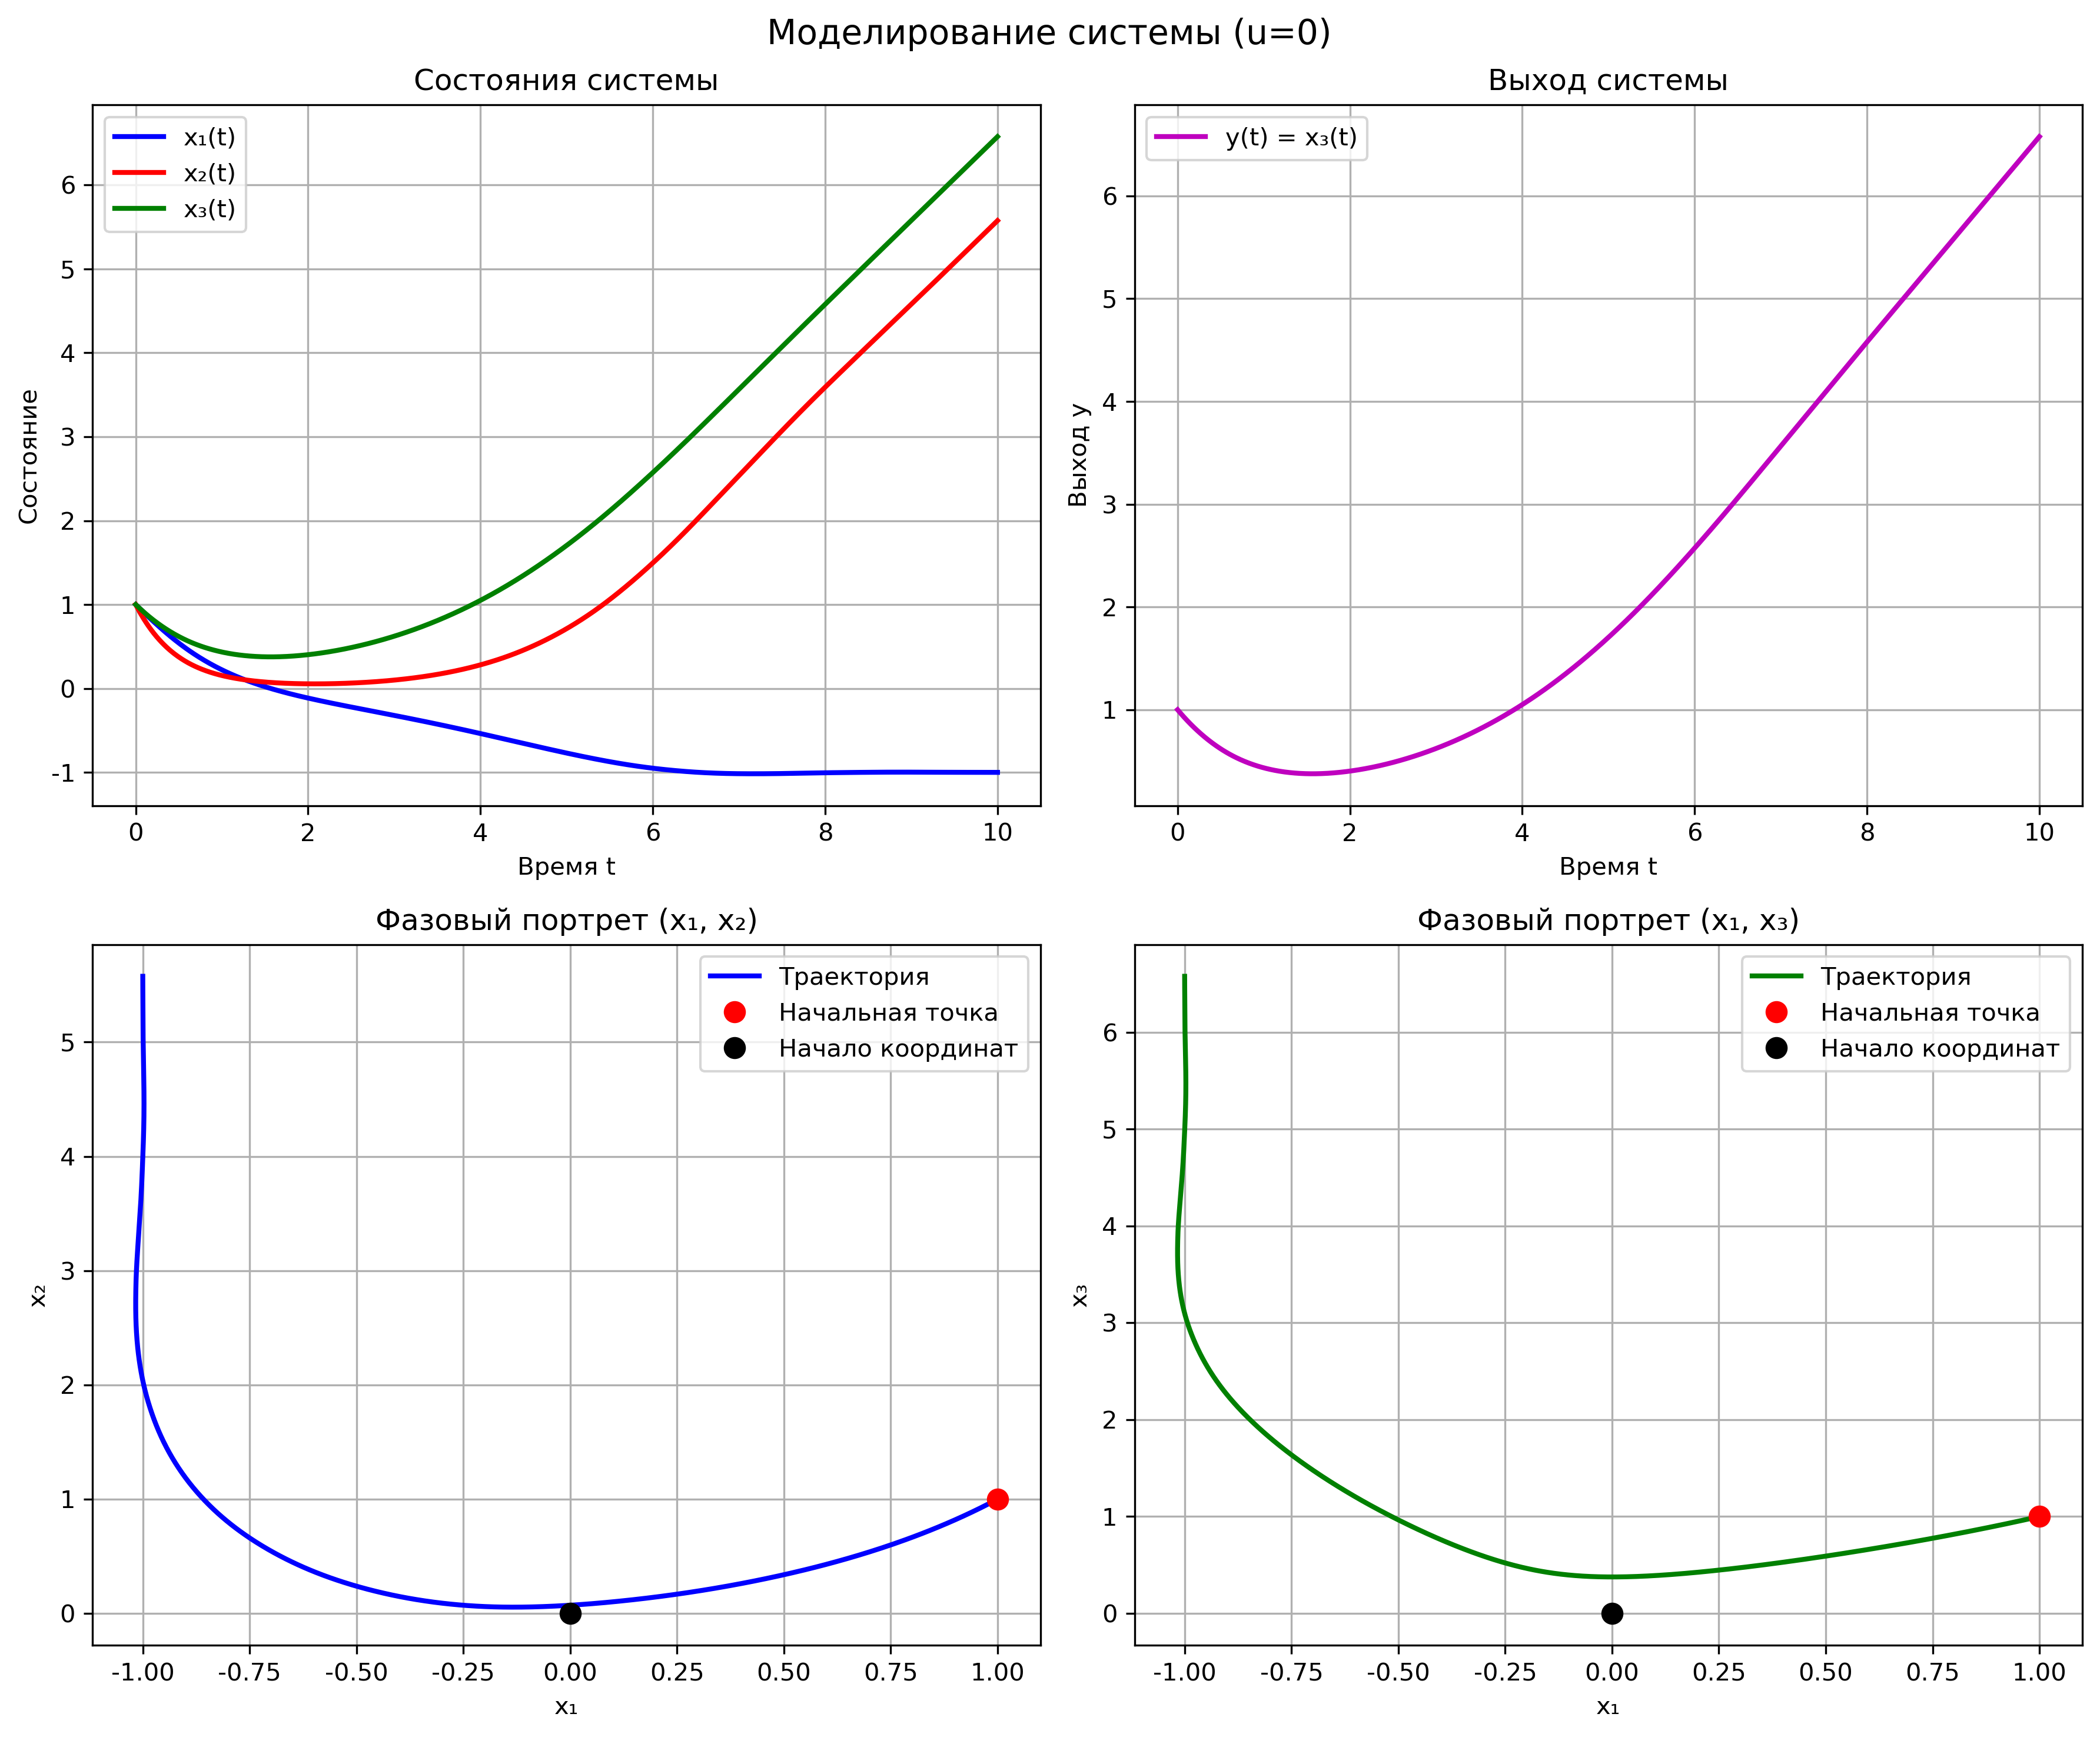
\includegraphics[width=0.9\textwidth]{task1/system_simulation.png}
\caption{Моделирование системы при нулевом управлении}
\label{fig:system_simulation}
\end{figure}

Результаты моделирования показывают поведение системы при нулевом управлении, демонстрируя внутреннюю динамику.

\subsection{Результаты задачи 1}

\textbf{Ответы:}
\begin{enumerate}
\item \textbf{Линеаризуемость:} Да, система линеаризуема по входу-выходу
\item \textbf{Относительная степень:} $r = 1$
\item \textbf{Нормальная форма:} получена с координатами $z_1 = x_3$, $z_2 = -x_1 + u$, $\eta_1 = x_1$, $\eta_2 = x_2$
\item \textbf{Область определения:} $\mathbb{R}^3$
\item \textbf{Минимально-фазовость:} Да, система минимально-фазовая
\end{enumerate}

\section{Задача 2. Синтез закона управления методом линеаризации обратной связью}

Рассмотрим систему:
\begin{align}
\dot{x}_1 &= -x_1 + x_2 \\
\dot{x}_2 &= x_1 - x_2 - x_1 x_3 + u \\
\dot{x}_3 &= x_1 + x_1 x_2 - 2x_3
\end{align}

Требуется найти закон управления с обратной связью по состоянию, обеспечивающий глобальную стабилизацию начала координат.

\subsection{Анализ управляемости}

Проверим управляемость системы через скобки Ли.

Векторное поле $g = [0, 1, 0]^T$ (коэффициенты при $u$).

Скобка Ли $[f, g] = \text{ad}_f g$:
\begin{align}
[f, g]_1 &= L_f g_1 - L_g f_1 = 0 - 0 = 0 \\
[f, g]_2 &= L_f g_2 - L_g f_2 = 0 - 1 = -1 \\
[f, g]_3 &= L_f g_3 - L_g f_3 = 0 - 0 = 0
\end{align}

Матрица управляемости в начале координат:
\begin{equation}
C = \begin{pmatrix} 0 & 0 & 0 \\ 1 & -1 & 0 \\ 0 & 0 & 0 \end{pmatrix}
\end{equation}

Ранг матрицы управляемости равен 2, что меньше размерности системы (3). Система не полностью управляема в начале координат.

\subsection{Проектирование регулятора}

Выберем выходную функцию $h(x) = x_1$ и применим метод линеаризации обратной связью.

\textbf{Шаг 1:} Вычисление производных Ли
\begin{align}
L_f h &= \frac{\partial h}{\partial x_1} f_1 + \frac{\partial h}{\partial x_2} f_2 + \frac{\partial h}{\partial x_3} f_3 \\
&= 1 \cdot (-x_1 + x_2) + 0 \cdot (x_1 - x_2 - x_1 x_3) + 0 \cdot (x_1 + x_1 x_2 - 2x_3) \\
&= -x_1 + x_2
\end{align}

\begin{align}
L_g L_f h &= \frac{\partial (L_f h)}{\partial x_1} g_1 + \frac{\partial (L_f h)}{\partial x_2} g_2 + \frac{\partial (L_f h)}{\partial x_3} g_3 \\
&= (-1) \cdot 0 + 1 \cdot 1 + 0 \cdot 0 = 1 \neq 0
\end{align}

Относительная степень $r = 2$.

\textbf{Шаг 2:} Синтез закона управления

Координаты нормальной формы:
\begin{align}
z_1 &= h = x_1 \\
z_2 &= L_f h = -x_1 + x_2
\end{align}

Вычисляем $L_f^2 h$:
\begin{align}
L_f^2 h &= \frac{\partial (L_f h)}{\partial x_1} f_1 + \frac{\partial (L_f h)}{\partial x_2} f_2 + \frac{\partial (L_f h)}{\partial x_3} f_3 \\
&= (-1) \cdot (-x_1 + x_2) + 1 \cdot (x_1 - x_2 - x_1 x_3) + 0 \cdot (x_1 + x_1 x_2 - 2x_3) \\
&= x_1 - x_2 + x_1 - x_2 - x_1 x_3 = 2x_1 - 2x_2 - x_1 x_3
\end{align}

Закон управления:
\begin{equation}
u = \frac{v - L_f^2 h}{L_g L_f h} = \frac{v - (2x_1 - 2x_2 - x_1 x_3)}{1} = v - 2x_1 + 2x_2 + x_1 x_3
\end{equation}

Выбираем $v = -k_1 z_1 - k_2 z_2 = -k_1 x_1 - k_2 (-x_1 + x_2)$ для стабилизации.

При $k_1 = 2$, $k_2 = 3$:
\begin{equation}
u = -2x_1 - 3(-x_1 + x_2) - 2x_1 + 2x_2 + x_1 x_3 = -x_1 - x_2 + x_1 x_3
\end{equation}

\subsection{Моделирование управляемой системы}

\begin{figure}[H]
\centering
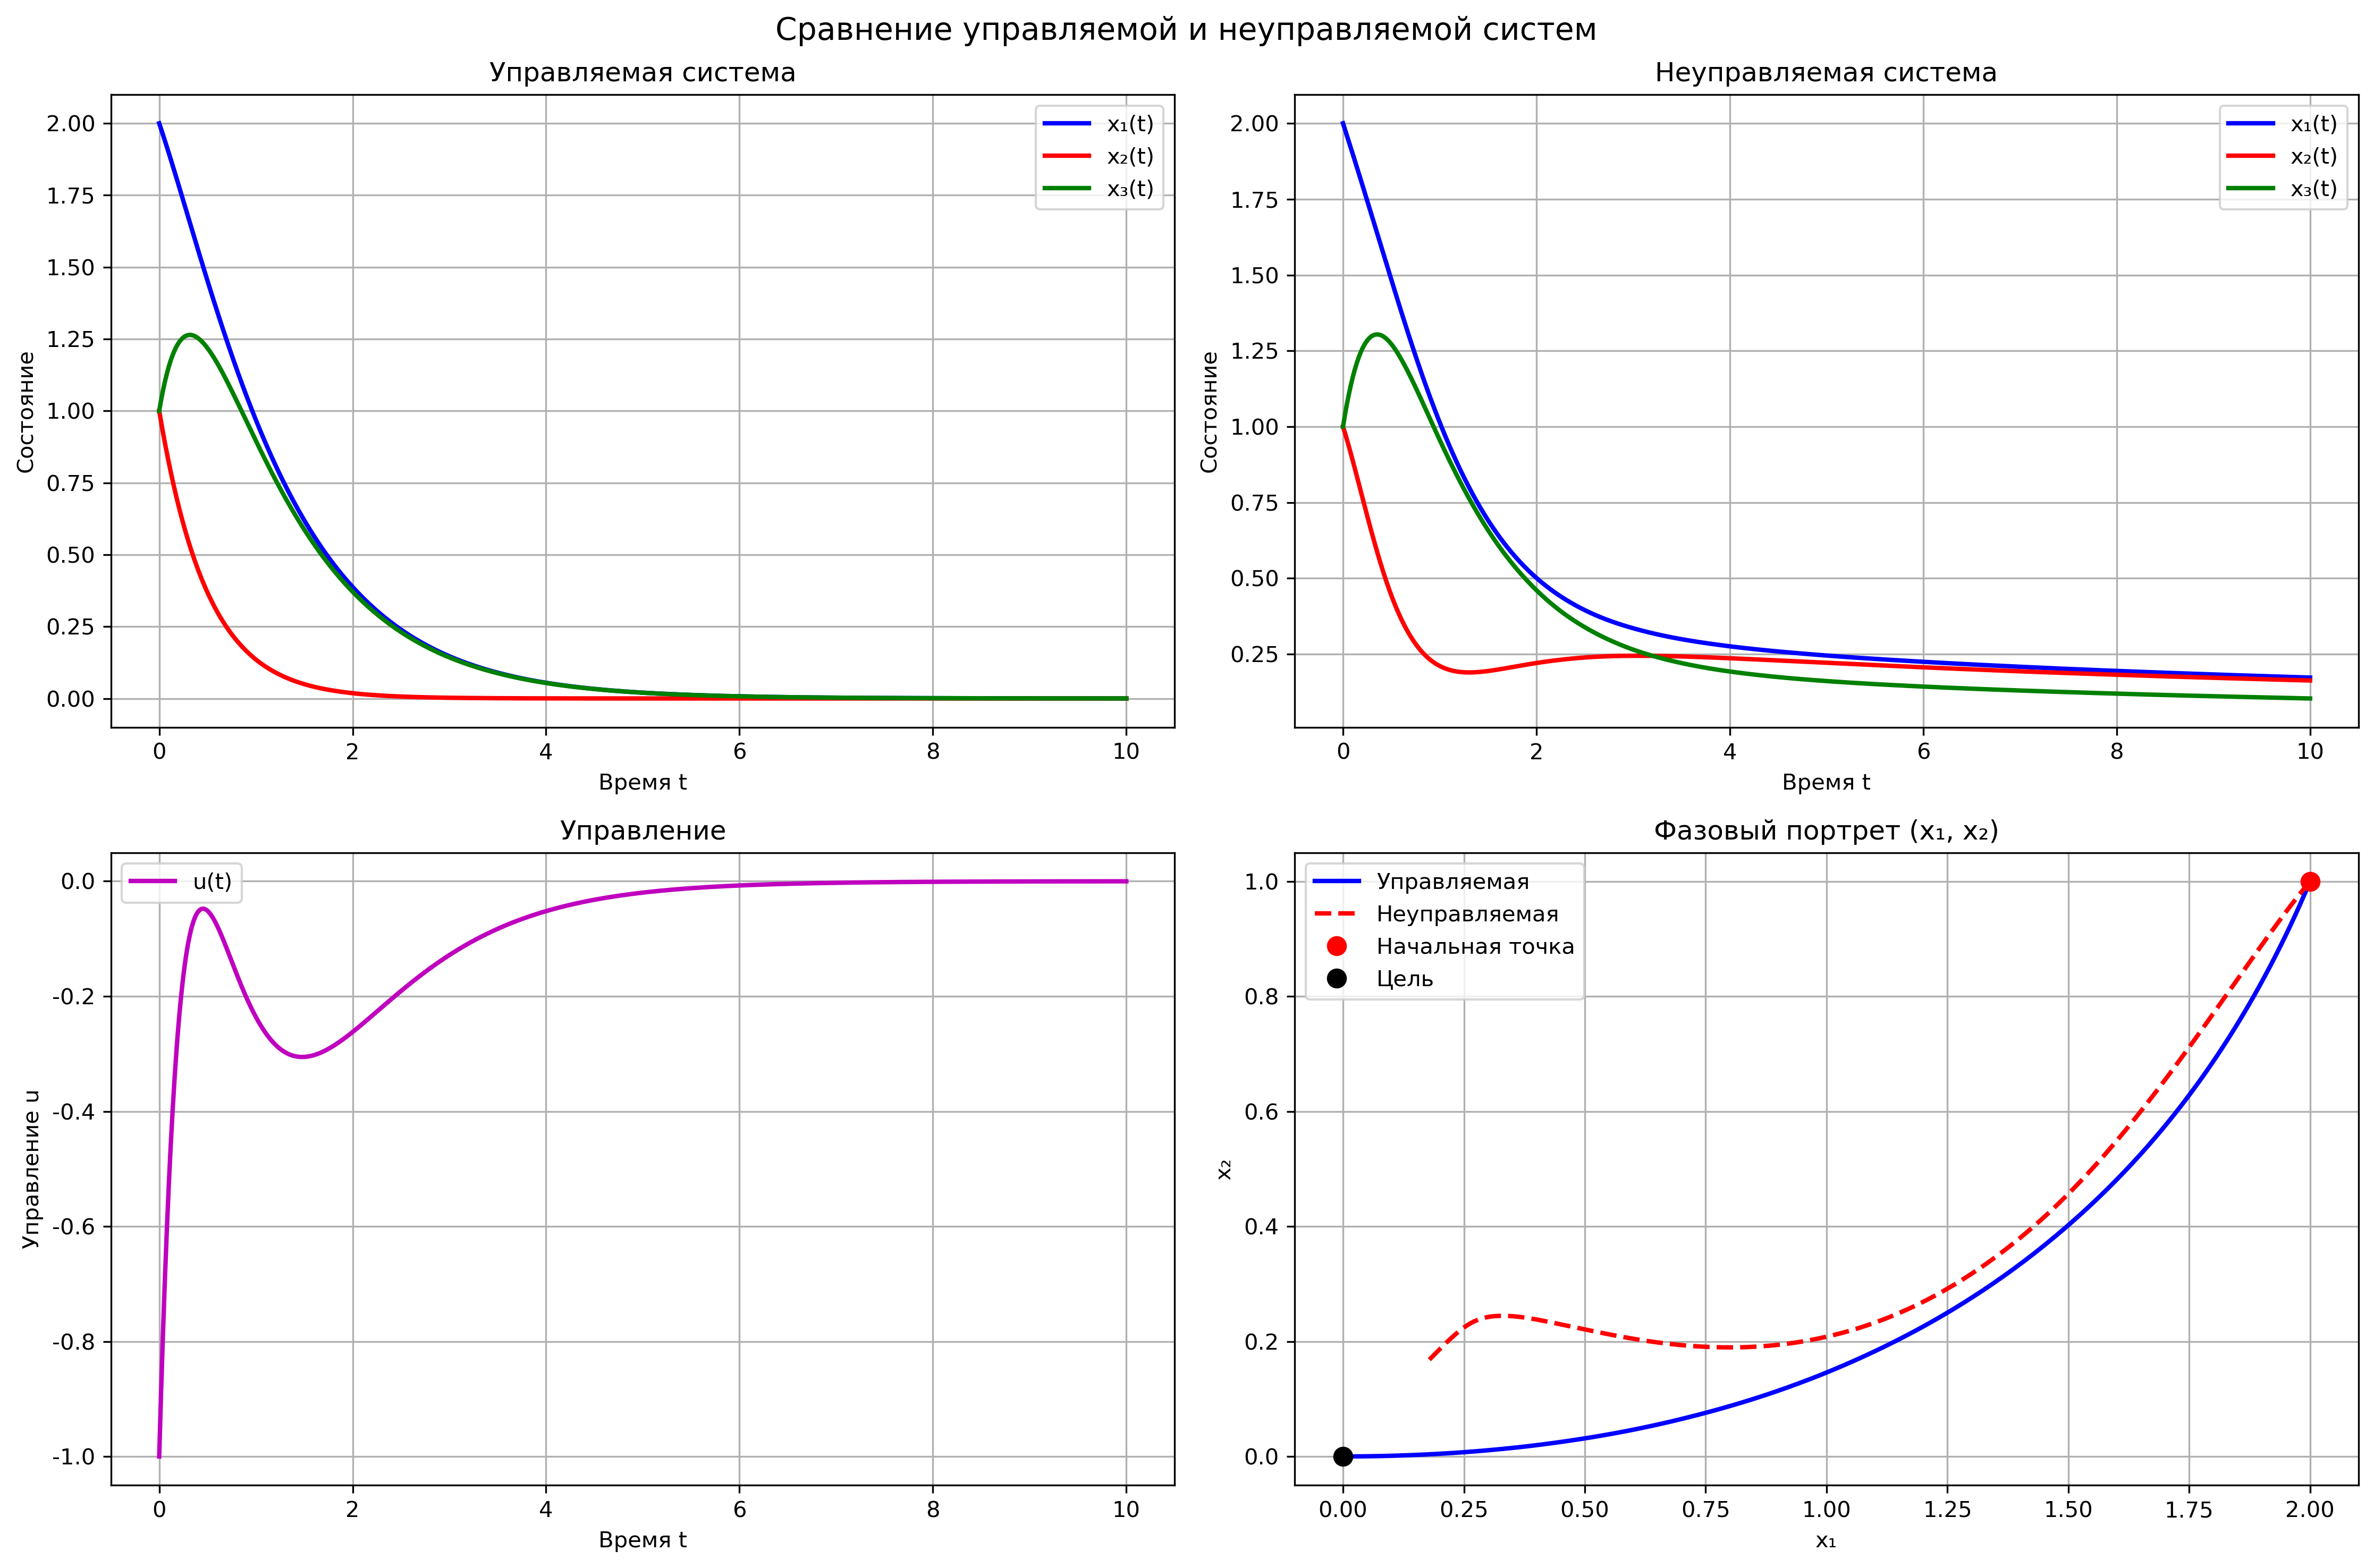
\includegraphics[width=0.9\textwidth]{task2/feedback_linearization.png}
\caption{Сравнение управляемой и неуправляемой систем}
\label{fig:feedback_linearization}
\end{figure}

Результаты моделирования показывают:
\begin{itemize}
\item Управляемая система экспоненциально сходится к началу координат
\item Неуправляемая система остается неустойчивой
\item Закон управления обеспечивает глобальную стабилизацию
\end{itemize}

\subsection{Результаты задачи 2}

\textbf{Закон управления:} $u = -x_1 - x_2 + x_1 x_3$

\textbf{Относительная степень:} $r = 2$

\textbf{Стабилизация:} Глобальная стабилизация начала координат достигнута

\section{Заключение}

В данной лабораторной работе были рассмотрены методы линеаризации обратной связью для нелинейных систем управления. Выполнены следующие задачи:

\begin{enumerate}
\item \textbf{Анализ линеаризуемости по входу-выходу:} для первой системы установлена линеаризуемость с относительной степенью $r = 1$ и минимально-фазовость.

\item \textbf{Преобразование в нормальную форму:} получены координаты нормальной формы с областью определения $\mathbb{R}^3$.

\item \textbf{Синтез закона управления:} для второй системы синтезирован закон управления $u = -x_1 - x_2 + x_1 x_3$, обеспечивающий глобальную стабилизацию начала координат.

\item \textbf{Численное моделирование:} подтверждена эффективность синтезированных законов управления.
\end{enumerate}

Работа продемонстрировала эффективность применения методов линеаризации обратной связью к практическим задачам управления нелинейными системами. Все поставленные задачи решены с использованием численного моделирования и визуализации результатов.
